\chapter{Preliminaries} \label{ch:prelim}

In the following we will  introduce the topics ... 


\begin{chapternotes}
  This chapter contains material previously published ...
\end{chapternotes}

\section{Basics}

This is my text with an example Figure~\ref{fig:example} and example
citation~\cite{Bringhurst1993} or \textcite{Bringhurst1993}. 

\begin{figure}
	\centering
	
\includegraphics[width=3cm]{institution}
	\caption{Example caption.}
	\label{fig:example}
\end{figure}

Now you are able to write your own document. Always keep in mind: it's
the \emph{content} that matters, not the form. But good typography is
able to deliver the content much better than information set with bad
typography. This template allows you to concentrate on writing good
content while the form is done by the template definitions.

\section{Additional Features}

You can use abbreviations using the \verb+\ac{}+ command like this: \ac{LTL}, 
where the abbreviation is expanded on first use and then printed normally: \ac{LTL}. 

Enumerations
\begin{enumerate}
	\item Foo
	\item Bar
\end{enumerate}

and itemizations
\begin{itemize}
	\item One
	\item Two
	\item Three
\end{itemize}

TikZ Pictures like in Figure~\ref{fig:def:prelim:ltl:kl-loop}
\begin{figure}
  \centering
  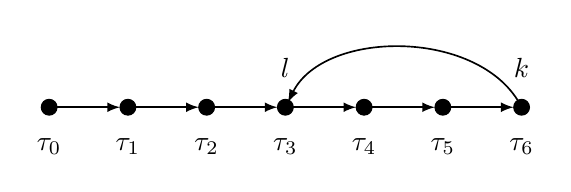
\begin{tikzpicture}
    \foreach \x in {0,1,2,3,4,5,6} 
    \draw[fill] (\x,5.5) circle (0.1);
    \foreach \x in {0,1,2,3,4,5} 
    \draw[-latex,semithick] (\x,5.5) -- +(0.9,0);
    \draw[-latex,shorten >=2,semithick] (6,5.5) .. controls (5.5,6.5) and (3.5,6.5) .. (3,5.5);
    \foreach \x in {0,1,2,3,4,5,6}
    \node at (\x,5) {$\tau_{\x}$};
    % \node at (-0.5,5) {$t=$};
    \node at (6,6) {$k$};
    \node at (3,6) {$l$};
  \end{tikzpicture}
  \caption{Some funny picture}
  \label{fig:def:prelim:ltl:kl-loop}
\end{figure}

Definitions:
\begin{definition}[Trace]\label{def:prelim:ltl:trace}
  I define that  $\tau = \Sigma$.
\end{definition}

Theorems:
\begin{theorem} \label{thm:enc:enc:basic}
	$\tau = \Sigma$ is true regardless of preconditions. 
\end{theorem}
\begin{proof}
with a proof \ldots 
\end{proof}

Lemmas:
\begin{lemma}
Doing X as follows does not affect the algorithm's correctness. 
\end{lemma}

Corollaries:
\begin{corollary} 
	No combination of the proposed modifications in the form of Lemmas X and Y and adopting H2 does affect the correctness of the algorithm.
\end{corollary}


Examples:

\begin{example} \label{ex:prelim:ltl:trace}
Lets do some silly example like to show that we are right \ldots
\end{example}

which can also be continued:

\begin{examplecont}{ex:prelim:ltl:trace}
	 like this and can contain figures which do not float outside the example 
	 environment like Figure~\ref{fig:prelim:ltl:exampletrace}.

	 \begin{fakefigure}
	  \vspace*{-1em}
		\centering
		\captionsetup{type=figure}
		
\includegraphics[width=5cm]{institution}
		\captionof{figure}{Example Figure}	
		\label{fig:prelim:ltl:exampletrace}
	\end{fakefigure}
\end{examplecont}

Tables: see Table~\ref{tab:example}.

\begin{table}
	\centering
	\begin{tabular}{llc}
	\toprule
	A & B & C\\
	\midrule
	1 & 2 & unknown\\
	x & y & z\\
	\bottomrule
	\end{tabular}
	\caption{Example Table}
	\label{tab:example}
\end{table}

Now you are able to write your own document. Always keep in mind: it's
the \emph{content} that matters, not the form. But good typography is
able to deliver the content much better than information set with bad
typography. This template allows you to concentrate on writing good
content while the form is done by the template definitions.